% 简洁风格：浅色背景 + 细边框 + 行号 + 自动换行
\definecolor{codebg}{RGB}{248,249,250}
\definecolor{codeframe}{RGB}{220,223,228}
\definecolor{codekw}{RGB}{25,85,145}
\definecolor{codecm}{RGB}{90,125,90}
\definecolor{codestr}{RGB}{136,44,136}

\lstdefinestyle{cleancpp}{
	language=C++,
	basicstyle=\ttfamily\small,
	keywordstyle=\bfseries\color{codekw},
    commentstyle=\color{codecm},
	stringstyle=\color{codestr},
	backgroundcolor=\color{codebg},
	frame=single,
	rulecolor=\color{codeframe},
	framesep=6pt,
	numbers=left,
	numberstyle=\scriptsize\color{gray},
	numbersep=8pt,
	breaklines=true,
	breakatwhitespace=false,
	showstringspaces=false,
	keepspaces=true,
	tabsize=4,
	columns=fullflexible
}


% Start here
\chapter{Exercise 3.1}

\section{Problem}

Give the recognized tokens of the following program in Pascal.

\begin{lstlisting}[style=cleancpp]
function max(i, j: integer): integer;
{return the maximum of integers i and j}
begin
	if i > j then max := i else max := j
end;
\end{lstlisting}

\section{Solution}

We need to recognize the tokens in the program, decomposing the program into a sequence of tokens. The token here means "词法单元" in Chinese.
In Pascal, every token can be represented as a tuple of the form \textbf{<Type, Value>}.


The value is the actual string that appears in the program, and there are several types of tokens in the program, including:

\begin{itemize}
	\item Reserved words: function, integer, return, begin, if, then, else, end
	\item Identifiers: max, i, j
	\item Punctuation: (, ), :, ;, {, }
	\item Operators: >, :=
	\item Constants: "return the maximum of integers i and j"
\end{itemize}

It's improtant to note that the comment in the program is not a token, so we can skip it when recognizing tokens.

The answer is as follow:

\begin{lstlisting}[style=cleancpp]
< Reserved words, function >
< Identifiers, max >
< Punctuation, ( >
< Identifiers, i >
< Punctuation, , >
< Identifiers, j >
< Punctuation, : >
< Reserved words, integer >
< Punctuation, ) >
< Punctuation, : >
< Reserved words, integer >
< Punctuation, ; >
(Skip the comment)
< Reserved words,begin >
< Reserved words, if >
< Identifiers, i >
< Operators, > >
< Identifiers, j >
< Reserved words, then >
< Identifiers, max >
< Operators, := >
< Identifiers, i >
< Reserved words, else >
< Identifiers, max >
< Operators, := >
< Identifiers, j >
< Reserved words, end >
< Punctuation, ; >
\end{lstlisting}


\chapter{Exercise 3.2}
\section{Problem}

(DBv2, Ch.3, pp.125, ex.3.3.2) 
Describethe languages denoted by the followingregular expressions:
\begin{lstlisting}[style=cleancpp]
a (a | b)* a
a* b a* b a* b a*
\end{lstlisting}

\section{Solution}

The first expression means the string that starts with "a", and end with "a".

The second expression means the string that only contains "a" and "b", and the number of "b" is only three.


\chapter{Exercise 3.3}
\section{Problem}

\begin{itemize}
	\item (DBv2, Ch.3, pp.125, ex.3.3.4) Most Languages are case sensitive, so keywords
		can be written only one way, and the regular expressions describing their
		lexemes are very simple
	\item However, some languages, like Pascal and SQL, are case insensitive. For example, the
		SQL keyword SELECT can also be written select, Select, or sELEcT.
	\item Show how to write a regular expression for a keyword in a case insensitive language.
		Illustrate your idea by writing the expression for SELECT in SQL.
\end{itemize}

\section{Solution}

We can write the expression for SELECT in the way as follow:

\begin{lstlisting}[style=cleancpp]
[Ss][Ee][Ll][Cc][Ee][Tt]
\end{lstlisting}

\chapter{Exercise 3.4}

\section{Problem}

Given the following regular expression

\begin{lstlisting}[style=cleancpp]
1*(0 | 01)*
\end{lstlisting}

\begin{enumerate}
	\item Transform it to an equivalent finite automaton.
	\item Construct an equivalent DFA for the result of exercise (1).
	\item Reduce the result of (2) and get a reduced DFA.
\end{enumerate}

\section{Solution}

\subsection{Problem 1}

The 1* represents the string that only contains "1".
The (0 | 01)* represents the string that only contains "0" or "01".
The number of the "1", "0", "01" is not limited, and also can be zero.

Therefore, the equivalent finite automaton can be represented as follow:
\begin{figure}[htbp]
	\centering
	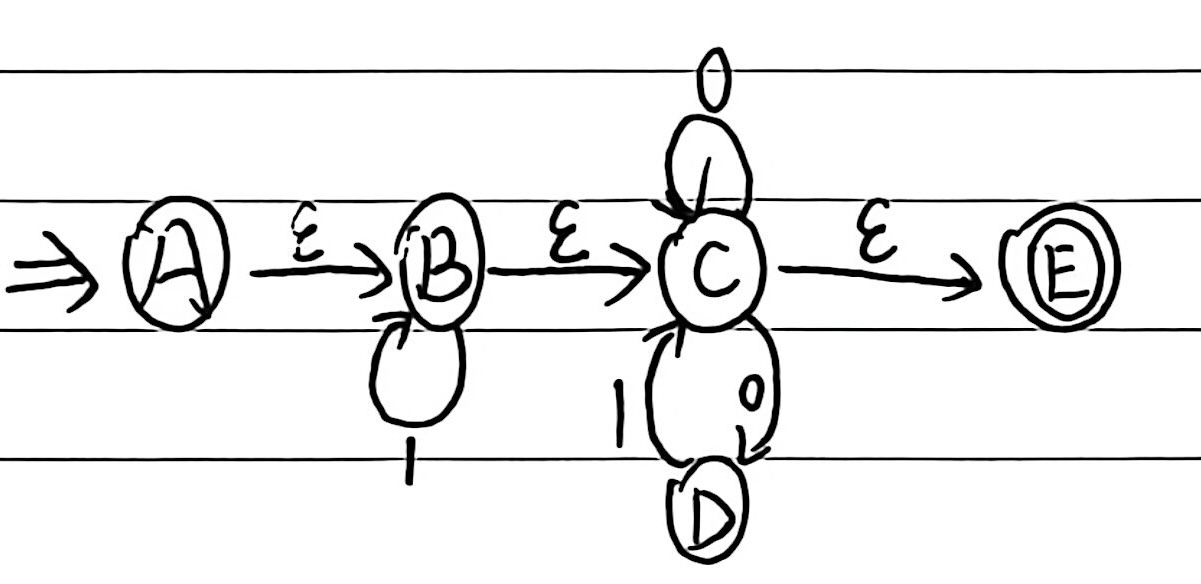
\includegraphics[width=0.6\textwidth]{image/e3_4_1.JPG}
\end{figure}

\subsection{Problem 2}

In order to transform the NFA to DFA, we should take the steps as follow:
\begin{itemize}
	\item The start state of the DFA is the epsilon-closure of the start state of the NFA, which is \{A, B, C, E\}.
	\item For each state in the DFA, we should calculate the epsilon-closure of the states that can be reached by the input symbol "0" and "1" respectively.
	\item Repeat the above steps until no new states can be added to the DFA.
	\item The accept states of the DFA are the states that contain the accept state of the NFA, which is \{A, B, C, E\}, \{C, D, E\}, \{B, C, E\}, \{C, E\}.And we can rename the states as X, Y, Z, W respectively.
\end{itemize}

\begin{figure}[htbp]
	\centering
	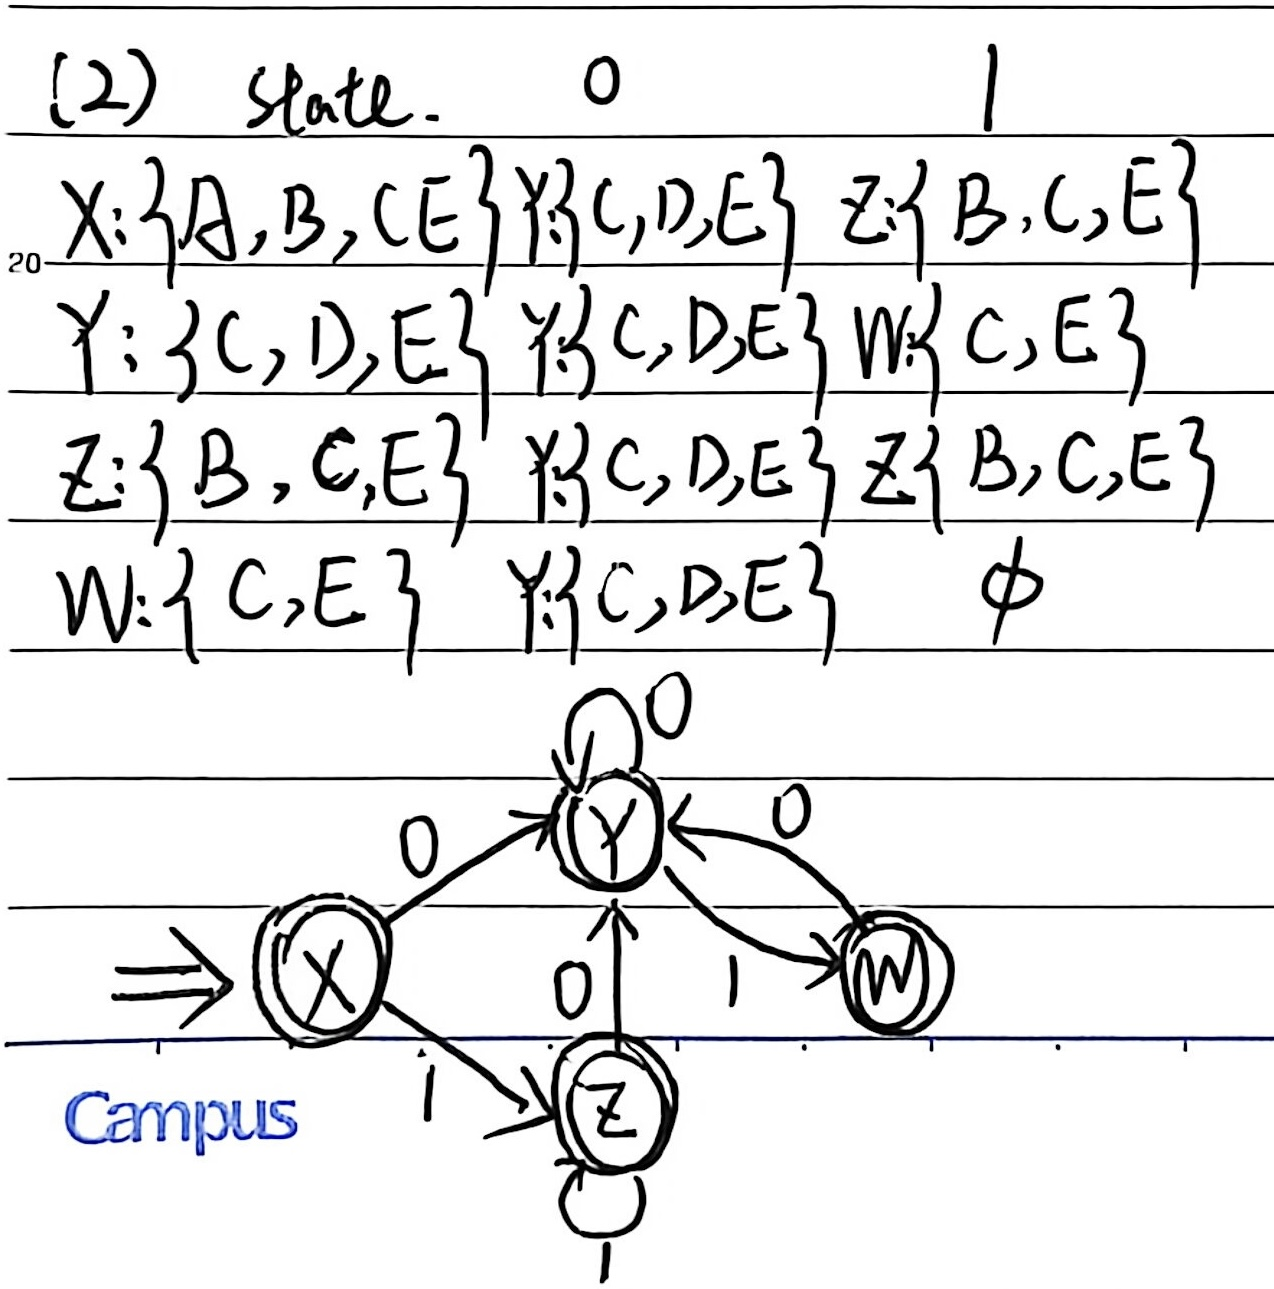
\includegraphics[width=0.6\textwidth]{image/e3_4_2.JPG}
\end{figure}

\subsection{Problem 3}

In order to reduce the DFA, we should take the steps as follow:
\begin{itemize}
	\item The states X, Y, Z, W are all double circles, which means they are all accept states. 
	\item In the set \{X, Y, Z, W \},"W" can produce $\phi$ via "1", which is not in the set \{X, Y, Z, W \}, so "W" should be separated from the other three states, renaming as "C".
	\item In the set \{X, Y, Z\}, "Y" can produce "W" via "1", which is not in the set \{X, Y, Z\}, so "Y" should be separated from the other two states, renaming as "B".
	\item In the set \{X, Z\}, no matter what the input symbol is, the next state is always in the set \{X, Z\}, so "X" and "Z" can be merged into one state, renaming as "A".
	\item So there are three states in the reduced DFA, which are "A", "B", "C".
\end{itemize}

\begin{figure}[htbp]
	\centering
	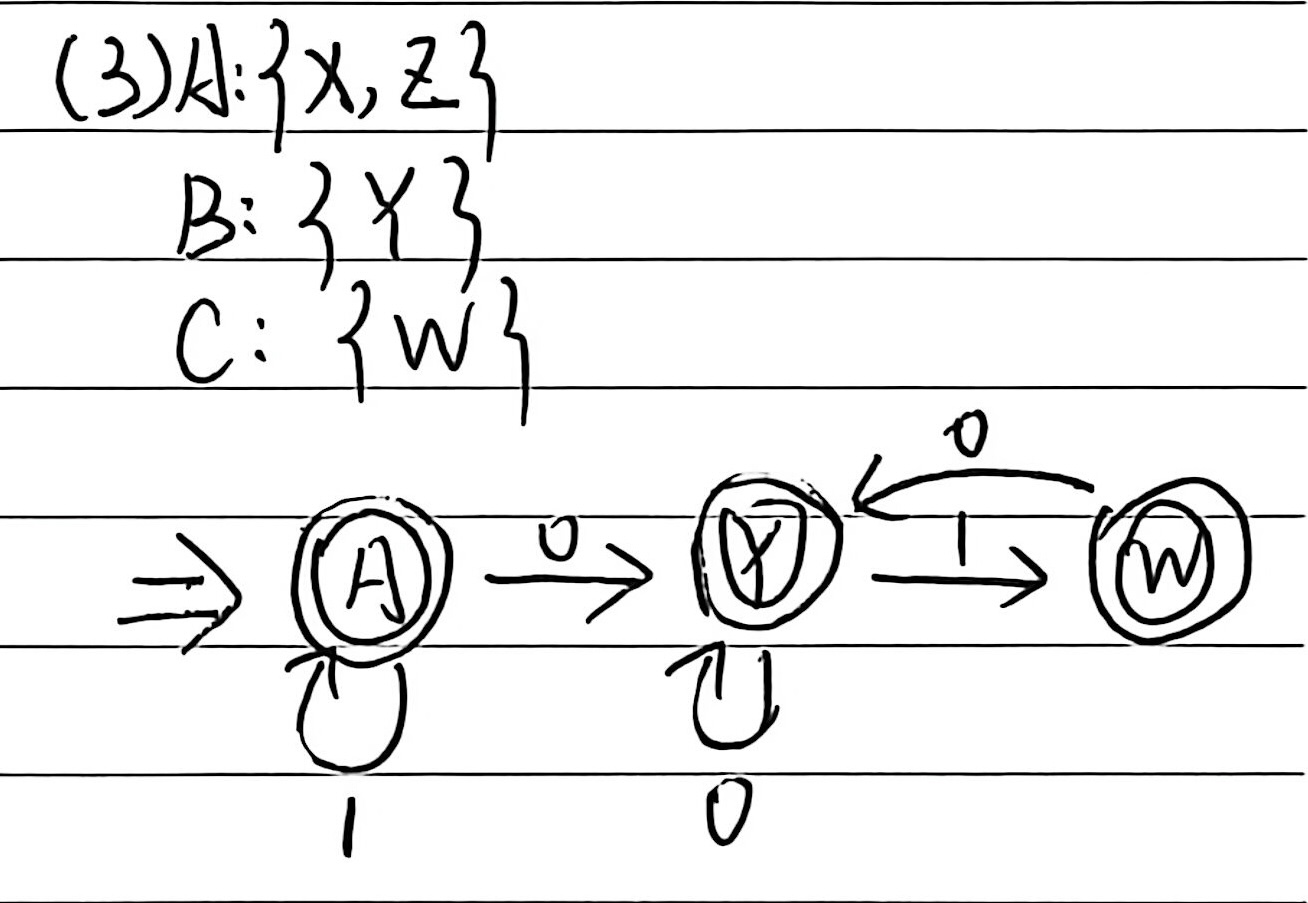
\includegraphics[width=0.6\textwidth]{image/e3_4_3.JPG}
\end{figure}

\chapter{Exercise 3.5**}

\section{Problem}

Given the alphabet $\Sigma$ = \{ z, o, / \}, a comment in a program over $\Sigma$ begins with "/o" and ends with "o/". Embedded comments are not permitted.

\begin{enumerate}
	\item Draw a DFA that recognizes nothing but all the comments in the source programs.
	\item Write a single regular expression that exactly describes all the comments in the source programs.
\end{enumerate}

\section{Solution}

\subsection{Problem 1}

The rules of the comments are as follow:
\begin{itemize}
	\item start with "/o"
	\item end with "o/"
	\item the content of the comment can only contain "z", "o", "/"
	\item the content of the comment can not contain "o/"
	\item "Embedded comments are not permitted" means that the content of the comment can contains "/o".
\end{itemize}

It's important to note that we don's consider the situation start with "//o" in this case, just focus on the comment with the format "/o...o/".
We can use the following table to represent the transition of the DFA
\begin{table}[htbp]
\centering
\begin{tabular}{c c c c}
\hline
State & Input $z$ & Input $o$ & Input $/$ \\
\hline
$S_0$ & $\phi$ & $\phi$ & $S_1$ \\
$S_1$ & $\phi$ & $S_2$ & $\phi$ \\
$S_2$ & $S_2$ & $S_3$ & $S_2$ \\
$S_3$ & $S_2$ & $S_3$ & $S_4$ \\
$S_4$ & $\phi$ & $\phi$ & $\phi$ \\
\hline
\end{tabular}

\end{table}

The DFA is as follow:
\begin{figure}[htbp]
	\centering
	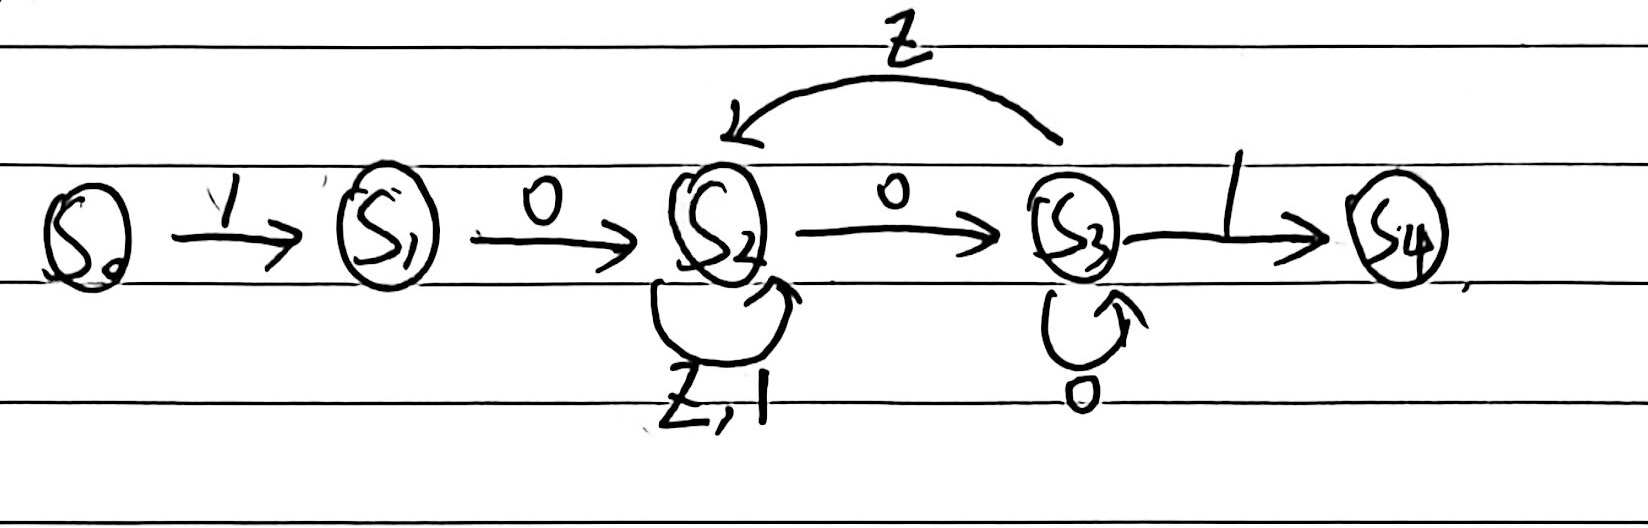
\includegraphics[width=0.5\textwidth]{image/e3_5_1.jpg}
\end{figure}

\subsection{Problem 2}

The problem can be interpreted as the string that starts with "/o", and end with "o/".It's in the format of "/o...content here...o/".
The content of the string can only contain "z", "o", "/", and the content of the string can not contain "o/".

The content in the comment can be represented as follow:

\begin{lstlisting}[style=cleancpp]
(z|/)* (o o* z (z|/)* )* o*
\end{lstlisting}

Add the start and end of the comment, we can get the regular expression as follow:

\begin{lstlisting}[style=cleancpp]
/o (z|/)* (o o* z (z|/)* )* o* o/
\end{lstlisting}
